\documentclass[usenames,dvipsnames,aspectratio=169]{beamer}
\usepackage{../common/prg}

\title[10. előadás]{Programozás}
\subtitle{(GKxB\_INTM114)}

\begin{document}

%1
\begin{frame}[plain]
  \titlepage
  \logoalul
\end{frame}

%2
\section{Projekt}
\subsection{Egy forrásfájlból álló program}
\begin{frame}
  Készítsünk programot, amely kezeli
  \begin{itemize}
    \item autók adatait:
    \begin{itemize}
      \item nyilvántartja: gyártás dátumát, utolsó műszaki vizsga dátumát, vizsgák darabszámát.
      \item kiszámítja: meddig érvényes a vizsga? (Az első 4 évre szól, minden későbbi 2-re.)
    \end{itemize}
    \item emberek adatait:
    \begin{itemize}
      \item nyilvántartja: nevet, születési dátumot.
      \item kiszámítja: elmúlt-e már 17 éves? (Kaphat-e ``B'' kat. jogosítványt?)
    \end{itemize}
    \item majd ezek felhasználásával kiszámítja:
    \begin{itemize}
      \item van jogosítvány + érv. műszaki v. $\to$ mehetünk autózni
      \item van jogosítvány + lejárt műszaki v. $\to$ le kell műszakiztatni az autót
      \item nincs jogosítvány $\to$ kicsit várunk még
    \end{itemize}
  \end{itemize}
\end{frame}

%3
\begin{frame}
  \begin{exampleblock}{\textattachfile{emberAuto1.cpp}{emberAuto1.cpp}}
    \small
    \vspace{-.2cm}
    \lstinputlisting[style=cpp,linerange={1-13},numbers=left,firstnumber=1]{emberAuto1.cpp}
    \vspace{-.2cm}
  \end{exampleblock}
\end{frame}

%4
\begin{frame}
  \begin{exampleblock}{\textattachfile{emberAuto1.cpp}{emberAuto1.cpp}}
    \vspace{-.2cm}
    \lstinputlisting[style=cpp,linerange={85-96},numbers=left,firstnumber=85]{emberAuto1.cpp}
    \vspace{-.2cm}
  \end{exampleblock}
\end{frame}

%5
\begin{frame}
  \begin{exampleblock}{\textattachfile{emberAuto1.cpp}{emberAuto1.cpp}}
    \vspace{-.2cm}
    \scriptsize
    \lstinputlisting[style=cpp,linerange={98-114},numbers=left,firstnumber=98]{emberAuto1.cpp}
    \vspace{-.2cm}
  \end{exampleblock}
\end{frame}

%6
\begin{frame}
  \begin{exampleblock}{\textattachfile{emberAuto1.cpp}{emberAuto1.cpp}}
    \vspace{-.2cm}
    \meret{7}
    \lstinputlisting[style=cpp,linerange={116-135},numbers=left,firstnumber=116]{emberAuto1.cpp}
    \vspace{-.2cm}
  \end{exampleblock}
\end{frame}

%7
\subsection{Több forrás- és fejfájlból álló program}
\begin{frame}
  Eddigi programjaink egyetlen forrásfájlból álltak, ld. \texttt{emberAuto1.cpp}\\
  Problémák:
  \begin{itemize}
    \item Áttekinthetetlenül nagyra nőnek a forrásszövegek
    \item Több programozó együttes munkája nehézkes
  \end{itemize}
  Megoldás:
  \begin{itemize}
    \item modularizáció: több fejfájl (\texttt{.h}, \texttt{.hpp}) és forrásfájl (\texttt{.cpp}) $\to$ egy program
    \begin{itemize}
      \item Fejfájlok: szimbolikus állandók, adattípusok (pl. struktúrák), fv. prototípusok
      \item Forrásfájlok: függvény definíciók
    \end{itemize}
    \item \{fej,forrás\}fájlok összekapcsolása: \emph{projekt} segítségével (ld. 
    make\hiv{\href{https://en.wikipedia.org/wiki/Make_(software)}{$^1$}$^{,}\,$\href{https://makefiletutorial.com/}{$^2$}}, 
    CMake\hiv{\href{https://en.wikipedia.org/wiki/CMake}{$^1$}$^{,}\,$\href{https://cmake.org/cmake/help/latest/guide/tutorial/index.html}{$^2$}},
    \hiv{\href{https://conan.io/}{Conan}})
  \end{itemize}
  Alakítsuk át az iménti programunkat!
\end{frame}

%8
\begin{frame}
  \footnotesize
  Régi módszer:\\
  \begin{alertblock}{\textattachfile{emberAuto1.cpp}{emberAuto1.cpp}}
    \texttt{bool szoko(int ev) \{ /* ... */ \}}\\
    \texttt{int napok(int ev, int ho) \{ /* ... */ \}}\\
    \texttt{bool ellenoriz(const datum* d) \{ /* ... */ \}}\\
    \texttt{int evNapja(const datum* d) \{ /* ... */ \}}\\
    \texttt{string hetNapja(const datum* d) \{ /* ... */ \}}\\
    \texttt{int bazis(const datum* d, int bazisEv=0) \{ /* ... */ \}}\\
    \texttt{int kulonbseg(const datum* tol, const datum* ig) \{ /* ... */ \}}\\
    \texttt{datum hoEsNap(int ev, int evNapja) \{ /* ... */ \}}\\
    \texttt{void nyomtat(const datum* d) \{ /* ... */ \}}\\
    \vspace{3mm}
    \texttt{bool elmult17(const ember* e, const datum* ma) \{ /* ... */ \}}\\
    \vspace{3mm}
    \texttt{datum muszakiErvenyesseg(const gepkocsi* gk) \{ /* ... */ \}}\\
    \vspace{3mm}
    \texttt{int main() \{ /* ... */ \}}\\
  \end{alertblock}
\end{frame}

%9
\begin{frame}
  \meret{7}
  Új módszer:\\
  \begin{columns}[c]
    \column{.5\textwidth}
      \hfill \texttt{\#include "ember2.h"} $\nearrow$ \\
      \hfill \texttt{\#include "datum2.h"} $\rightarrow$ \\
      \hfill \texttt{\#include "gepkocsi2.h"} $\searrow$ \\
      \begin{exampleblock}{\textattachfile{emberAuto2.cpp}{emberAuto2.cpp}}
        \texttt{int main() \{ /* ... */ \}}\\
      \end{exampleblock}
    \column{.5\textwidth}
      \begin{exampleblock}{\textattachfile{ember2.h}{ember2.h}}
        \texttt{bool elmult17(const ember* e, const datum* ma);}\\
      \end{exampleblock}
      $\downarrow$ \texttt{\#include "datum2.h"}\\
      \begin{exampleblock}{\textattachfile{datum2.h}{datum2.h}}
        \texttt{bool szoko(int ev);}\\
        \texttt{int napok(int ev, int ho);}\\
        \texttt{bool ellenoriz(const datum* d);}\\
        \texttt{int evNapja(const datum* d);}\\
        \texttt{string hetNapja(const datum* d);}\\
        \texttt{int bazis(const datum* d, int bazisEv);}\\
        \texttt{int kulonbseg(const datum* tol, const datum* ig);}\\
        \texttt{datum hoEsNap(int ev, int evNapja);}\\
        \texttt{void nyomtat(const datum* d);}\\
      \end{exampleblock}
      $\uparrow$ \texttt{\#include "datum2.h"}\\
      \begin{exampleblock}{\textattachfile{gepkocsi2.h}{gepkocsi2.h}}
        \texttt{datum muszakiErvenyesseg(const gepkocsi* gk);}\\
      \end{exampleblock}
  \end{columns}
\end{frame}

%10
\begin{frame}
  Régi módszer:\\
  \begin{alertblock}{Fordítás (compile)}
    \texttt{g++ -Wall -c emberAuto1.cpp}\\
  \end{alertblock}
  \begin{alertblock}{Kapcsoló-szerkesztés (link)}
    \texttt{g++ -o emberAuto1 emberAuto1.o}\\
  \end{alertblock}
  \vfill
  \begin{alertblock}{Összeállítás (build)}
    \texttt{g++ -Wall -o emberAuto1 emberAuto1.cpp}\\
  \end{alertblock}
\end{frame}

%11
\begin{frame}
  Új módszer:\\
  \begin{exampleblock}{Fordítás (compile)}
    \texttt{g++ -Wall -c datum2.cpp ember2.cpp gepkocsi2.cpp emberAuto2.cpp}\\
  \end{exampleblock}
  \begin{exampleblock}{Kapcsoló-szerkesztés (link)}
    \texttt{g++ -Wall -c datum2.cpp ember2.cpp gepkocsi2.cpp emberAuto2.cpp}\\
  \end{exampleblock}
  \vfill
  \begin{exampleblock}{Összeállítás (build)}
    \footnotesize
    \texttt{g++ -Wall -o emberAuto2 datum2.cpp ember2.cpp gepkocsi2.cpp emberAuto2.cpp}\\
  \end{exampleblock}
\end{frame}

%12
\begin{frame}[fragile]
  \meret{7}
  \begin{alertblock}{Probléma: újradefiniált típus}
    \vspace{-.2cm}
    \begin{verbatim}
g++ -Wall -o emberAuto2 datum2.cpp ember2.cpp gepkocsi2.cpp emberAuto2.cpp
In file included from gepkocsi2.h:3,
                  from emberAuto2.cpp:2:
datum2.h:8:8: error: redefinition of 'struct datum'
    8 | struct datum {
      |        ^~~~~
In file included from ember2.h:3,
                  from emberAuto2.cpp:1:
datum2.h:8:8: note: previous definition of 'struct datum'
    8 | struct datum {
      |        ^~~~~
In file included from emberAuto2.cpp:3:
datum2.h:8:8: error: redefinition of 'struct datum'
    8 | struct datum {
      |        ^~~~~
In file included from ember2.h:3,
                  from emberAuto2.cpp:1:
datum2.h:8:8: note: previous definition of 'struct datum'
    8 | struct datum {
      |        ^~~~~
\end{verbatim}
    \vspace{-.2cm}
  \end{alertblock}
\end{frame}

%13
\begin{frame}
  \begin{center}
    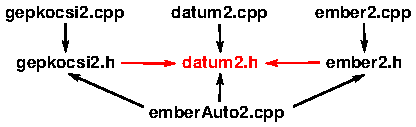
\includegraphics[scale=1.25]{emberAuto2.pdf}
  \end{center}
  \vfill
  Források: \textattachfile{gepkocsi2.cpp}{gepkocsi2.cpp}, \textattachfile{datum2.cpp}{datum2.cpp}, \textattachfile{ember2.cpp}{ember2.cpp}, \textattachfile{emberAuto2.cpp}{emberAuto2.cpp}\\
  Fejfájlok: \textattachfile{gepkocsi2.h}{gepkocsi2.h}, \textattachfile{datum2.h}{datum2.h}, \textattachfile{ember2.h}{ember2.h}\\
\end{frame}

%14
\subsection{Feltételes fordítás, header guard}
\begin{frame}[fragile]
  Feltételes fordítás: feltételektől függően bizonyos programrészek megőrzése/kihagyása
  \begin{exampleblock}{Feltétles fordítás}
    \begin{verbatim}
#if konstans-kifejezés1 <szekció1>
<#elif konstans-kifejezés2 <szekció2>>
/* ... */
<#elif konstans-kifejezésN <szekcióN>>
<#else <végső-szekció>>
#endif
\end{verbatim}
  \end{exampleblock}
  \begin{itemize}
    \item A \texttt{konstans-kifejezés}ek típusa logikainak tekintendő.
    \item Csak karakter és egész állandókat, \texttt{defined} operátort tartalmazhat
  \end{itemize}
\end{frame}

%15
\begin{frame}[fragile]
  \small
  A \texttt{defined} operátor
  \begin{itemize}
    \item célja: makrók definiáltságát ellenőrzi
    \item alakjai:\\
\texttt{defined(\emph{azonosító})}\\
\texttt{defined \emph{azonosító}}
    \item eredmény: logikai, és logikai operátorokkal együtt használható
    \item alkalmazása: pl. biztosíthatja, hogy egy fejfájl egyszer kerülhessen csak beépítésre (\kiemel{include/header guard}), platform-specifikus megoldások közül egynek a használata
  \end{itemize}
  \begin{exampleblock}{\texttt{fej.h}}
    \vspace{-.4cm}
    \begin{verbatim}
#if !defined(FEJ)
  #define FEJ
  /* érdemi tartalom */
#endif
\end{verbatim}
    \vspace{-.3cm}
  \end{exampleblock}
\end{frame}

%16
\begin{frame}[fragile]
  Az \texttt{\#ifdef, \#ifndef} direktívák
  \begin{itemize}
    \item céljuk: makró definiáltságát/definiálatlanságát ellenőrzik
    \item \texttt{\#if defined(\emph{azonosító})} $\equiv$ \texttt{\#ifdef \emph{azonosító}}
    \item \texttt{\#if !defined(\emph{azonosító})} $\equiv$ \texttt{\#ifndef \emph{azonosító}}
  \end{itemize}
    \begin{exampleblock}{\texttt{fej.h}}
    \begin{verbatim}
#ifndef FEJ
  #define FEJ
  /* érdemi tartalom */
#endif
\end{verbatim}
  \end{exampleblock}
\end{frame}

%17
\begin{frame}
  \meret{7}
  \begin{exampleblock}{\textattachfile{datum3.h}{datum3.h}}
    \vspace{-.2cm}
    \lstinputlisting[style=cpp,linerange={1-15},numbers=left,firstnumber=1]{datum3.h}
    \lstinputlisting[style=cpp,linerange={23-25},numbers=left,firstnumber=23]{datum3.h}
    \vspace{-.2cm}
  \end{exampleblock}
  \textattachfile{datum3.cpp}{datum3.cpp}, \textattachfile{ember3.cpp}{ember3.cpp}, \textattachfile{ember3.h}{ember3.h}, 
  \textattachfile{gepkocsi3.cpp}{gepkocsi3.cpp}, \textattachfile{gepkocsi3.h}{gepkocsi3.h}, 
  \textattachfile{emberAuto3.cpp}{emberAuto3.cpp}
\end{frame}

%18
\section{Absztrakt adatszerkezetek -- megvalósítás tömbökkel}
\subsection{Verem}
\begin{frame}
  Verem (stack)
  \begin{itemize}
    \item LIFO (Last In, First Out) szervezésű tár: tárolás sorrendjével ellentétes sorrendben férünk hozzá az adatokhoz
    \item Műveletek: berak (push), kivesz (pop), kukucskál (peek), ürít (clear), \dots
    \item Alkalmazási terület: pl. böngészési előzmények listája (history) egy webböngészőben
  \end{itemize}
  \begin{center}
    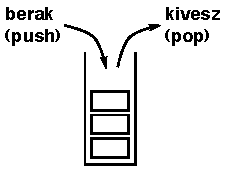
\includegraphics{verem.pdf}
  \end{center}
\end{frame}

%19
\begin{frame}
  \begin{exampleblock}{\textattachfile{verem1.h}{verem1.h}}
    \vspace{-.2cm}
    \lstinputlisting[style=cpp,numbers=left]{verem1.h}
    \vspace{-.2cm}
  \end{exampleblock}
\end{frame}

%20
\begin{frame}
  \scriptsize
  \begin{exampleblock}{\textattachfile{verem1.cpp}{verem1.cpp}}
    \vspace{-.2cm}
    \lstinputlisting[style=cpp,numbers=left,linerange={1-16}]{verem1.cpp}
    \vspace{-.2cm}
  \end{exampleblock}
\end{frame}

%21
\begin{frame}
  \begin{exampleblock}{\textattachfile{verem1.cpp}{verem1.cpp}}
    \vspace{-.2cm}
    \lstinputlisting[style=cpp,numbers=left,linerange={18-29},firstnumber=18]{verem1.cpp}
    \vspace{-.2cm}
  \end{exampleblock}
\end{frame}

%22
\begin{frame}[fragile]
  \small
  \begin{columns}[c]
    \column{0.47\textwidth}
    \begin{exampleblock}{\textattachfile{veremTeszt1.cpp}{veremTeszt1.cpp}}
      \vspace{-.2cm}
      \lstinputlisting[style=cpp,numbers=left]{veremTeszt1.cpp}
      \vspace{-.2cm}
    \end{exampleblock}
    \column{0.47\textwidth}
    \begin{block}{Kimenet}
      \begin{verbatim}
citrom
barack
alma
\end{verbatim}
    \end{block}
  \end{columns}
\end{frame}

%23
\subsection{Sor}
\begin{frame}
  Sor (queue)
  \begin{itemize}
    \item First In First Out (FIFO) adatszerkezet
    \item Alkalmazása: pl. felhasználók egymás után küldenek nyomtatási feladatokat, amiket a nyomtató a sorba rakás sorrendjében hajt végre
  \end{itemize}
  \footnotesize
  \begin{exampleblock}{\textattachfile{sor1.h}{sor1.h}}
    \vspace{-.3cm}
    \lstinputlisting[style=cpp,numbers=left]{sor1.h}
    \vspace{-.3cm}
  \end{exampleblock}
\end{frame}

%24
\begin{frame}
  \scriptsize
  \begin{exampleblock}{\textattachfile{sor1.cpp}{sor1.cpp}}
    \vspace{-.3cm}
    \lstinputlisting[style=cpp,linerange={1-19},numbers=left]{sor1.cpp}
    \vspace{-.3cm}
  \end{exampleblock}
\end{frame}

%25
\begin{frame}
  \footnotesize
  \begin{exampleblock}{\textattachfile{sor1.cpp}{sor1.cpp}}
    \lstinputlisting[style=cpp,linerange={21-34},numbers=left,firstnumber=21]{sor1.cpp}
  \end{exampleblock}
\end{frame}

%26
\begin{frame}
  \scriptsize
  \begin{exampleblock}{\textattachfile{sorTeszt1.cpp}{sorTeszt1.cpp}}
    \lstinputlisting[style=cpp,numbers=left]{sorTeszt1.cpp}
  \end{exampleblock}
\end{frame}

%27
\begin{frame}
  \begin{center}
    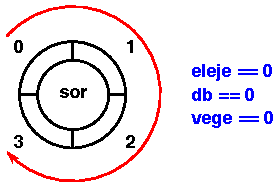
\includegraphics[scale=1.5]{sor/sor01.pdf}
  \end{center}
\end{frame}

%28
\begin{frame}
  \begin{center}
    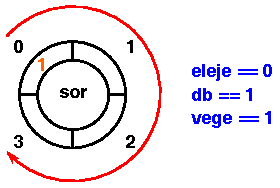
\includegraphics[scale=1.5]{sor/sor02.pdf}
  \end{center}
\end{frame}

%29
\begin{frame}
  \begin{center}
    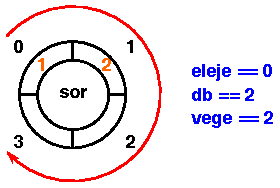
\includegraphics[scale=1.5]{sor/sor03.pdf}
  \end{center}
\end{frame}

%30
\begin{frame}
  \begin{center}
    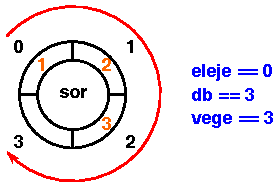
\includegraphics[scale=1.5]{sor/sor04.pdf}
  \end{center}
\end{frame}

%31
\begin{frame}
  \begin{center}
    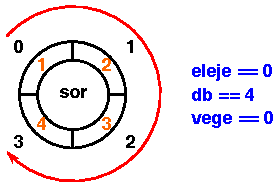
\includegraphics[scale=1.5]{sor/sor05.pdf}
  \end{center}
\end{frame}

%32
\begin{frame}
  \begin{center}
    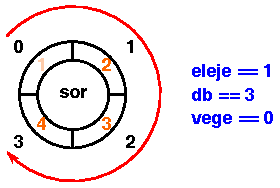
\includegraphics[scale=1.5]{sor/sor06.pdf}
  \end{center}
\end{frame}

%33
\begin{frame}
  \begin{center}
    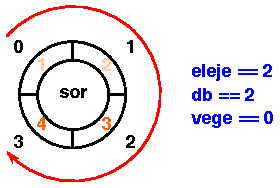
\includegraphics[scale=1.5]{sor/sor07.pdf}
  \end{center}
\end{frame}

%34
\begin{frame}
  \begin{center}
    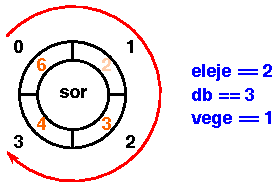
\includegraphics[scale=1.5]{sor/sor08.pdf}
  \end{center}
\end{frame}

%35
\begin{frame}
  \begin{center}
    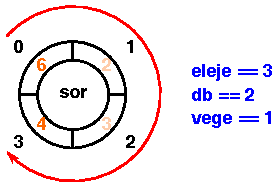
\includegraphics[scale=1.5]{sor/sor09.pdf}
  \end{center}
\end{frame}

%36
\begin{frame}
  \begin{center}
    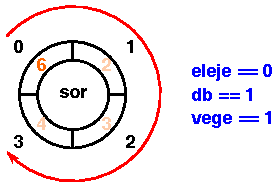
\includegraphics[scale=1.5]{sor/sor10.pdf}
  \end{center}
\end{frame}

%37
\begin{frame}
  \begin{center}
    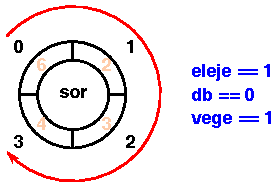
\includegraphics[scale=1.5]{sor/sor11.pdf}
  \end{center}
\end{frame}

\end{document}